\documentclass[11pt,a4paper]{article}

\usepackage[margin=0.78in]{geometry}
\usepackage[T1]{fontenc}
\usepackage{lmodern}
\usepackage{microtype}
\usepackage{setspace}
\usepackage{enumitem}
\usepackage{booktabs}
\usepackage{array}
\usepackage{tikz}
\usetikzlibrary{arrows.meta,positioning,shapes.geometric,fit,calc}
\usepackage{titlesec}
\usepackage{caption}
\usepackage[hidelinks]{hyperref}

\setstretch{1.03}
\setlength{\parindent}{0pt}
\setlength{\parskip}{4pt}
\setlist[itemize]{leftmargin=1.45em,itemsep=1pt,topsep=2pt}
\setlist[enumerate]{leftmargin=1.55em,itemsep=1pt,topsep=2pt}

\titleformat{\section}{\Large\bfseries}{\thesection}{0.65em}{}
\titleformat{\subsection}{\large\bfseries}{\thesubsection}{0.65em}{}
\titlespacing*{\section}{0pt}{10pt}{3pt}
\titlespacing*{\subsection}{0pt}{7pt}{2pt}

\tikzset{
 box/.style={draw,rounded corners=2pt,align=center,minimum height=0.62cm,
             minimum width=2.35cm,font=\small},
 arrow/.style={-{Latex[length=2mm]},thick},
 smallbox/.style={draw,rounded corners=2pt,align=center,minimum height=0.55cm,
             minimum width=1.85cm,font=\scriptsize}
}

\begin{document}

% ---------------- Header ----------------
\begin{center}
{\LARGE\bfseries HyperTrack: Hyperhidrosis Monitoring and Management System\par}
\vspace{2pt}
{\large Project Proposal for UCS503\par}
{\large Submitted to: Dr. Jeelani Asif\par}
{\large Thapar Institute of Engineering and Technology\par}
\vspace{9pt}
Prabhkirat Kaur, DSAI \hspace{1.1cm} Aditya Rajput, DSAI\par
\vspace{4pt}
{\large August 2026\par}
\end{center}

\section{Higher-order goal}

HyperTrack aims to improve the consistency and usefulness of hyperhidrosis symptom monitoring by reducing the manual effort required to record sweating episodes and understand patterns over time. The immediate engineering goal is to turn user-recorded, structured data into a reliable monitoring, analytics, and reporting workflow.

\begin{center}
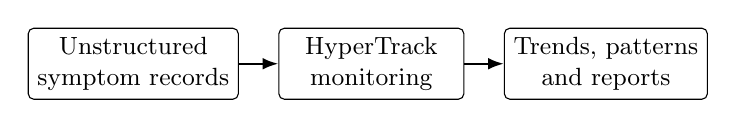
\begin{tikzpicture}[node distance=5mm]
\node[box] (problem) {Unstructured\\symptom records};
\node[box,right=of problem] (track) {HyperTrack\\monitoring};
\node[box,right=of track] (insight) {Trends, patterns\\and reports};
\draw[arrow] (problem)--(track);
\draw[arrow] (track)--(insight);
\end{tikzpicture}
\captionof{figure}{Problem context and motivation for structured monitoring.}
\end{center}


\section{Time-to-value}

\begin{itemize}
\item Build the core record--store--analyze--report workflow first and add advanced ML features later.
\item Deliver incremental functionality through short development iterations and continuous testing.
\item Measure usefulness through recording completeness, dashboard functionality, report generation, and ML evaluation where implemented.
\end{itemize}


\section{Problem Statement}

Hyperhidrosis can involve excessive sweating of areas such as the palms, feet, underarms, and face. A practical challenge is the lack of consistent records covering severity, duration, affected area, activity, stress, and possible triggers. Without structured history, users may find it difficult to identify recurring patterns.

HyperTrack addresses this gap by allowing users to record episodes in a structured database, visualize historical trends, and generate an organized monitoring report. The system is a monitoring and decision-support tool; it does not diagnose or treat hyperhidrosis.


\section{Objectives}

\begin{itemize}
\item Provide a simple interface for recording sweating episodes and context.
\item Store records securely in a structured relational database.
\item Analyze frequency, severity, duration, affected areas, and possible triggers.
\item Provide dashboards with statistics and historical trends.
\item Support treatment/session tracking without issuing prescriptions.
\item Generate an organized monitoring report.
\item Investigate supervised ML for personalized severity prediction.
\item Apply software engineering practices across analysis, design, development, and testing.
\end{itemize}


\section{Proposed Solution}

The proposed web application contains eight core modules:

\begin{center}
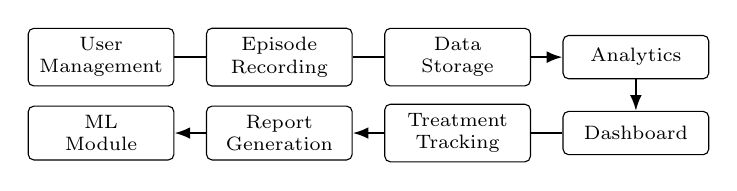
\begin{tikzpicture}[node distance=4mm and 4mm]
\node[smallbox] (u) {User\\Management};
\node[smallbox,right=of u] (e) {Episode\\Recording};
\node[smallbox,right=of e] (d) {Data\\Storage};
\node[smallbox,right=of d] (a) {Analytics};
\node[smallbox,below=of a] (dash) {Dashboard};
\node[smallbox,left=of dash] (t) {Treatment\\Tracking};
\node[smallbox,left=of t] (r) {Report\\Generation};
\node[smallbox,left=of r] (ml) {ML\\Module};
\draw[arrow] (u)--(e)--(d)--(a);
\draw[arrow] (a)--(dash);
\draw[arrow] (dash)--(t)--(r);
\draw[arrow] (r)--(ml);
\end{tikzpicture}
\captionof{figure}{Core functional modules of HyperTrack.}
\end{center}


\section{System Architecture}

The system follows a three-tier architecture. The presentation layer provides the interface, the application layer handles APIs, analytics and ML services, and the data layer stores users, episodes, triggers and treatment records.

\begin{center}
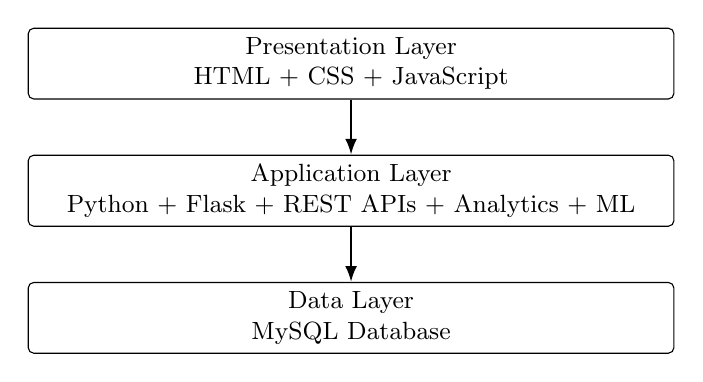
\begin{tikzpicture}[node distance=7mm]
\node[box,minimum width=8.2cm] (p) {Presentation Layer\\HTML + CSS + JavaScript};
\node[box,minimum width=8.2cm,below=of p] (app) {Application Layer\\Python + Flask + REST APIs + Analytics + ML};
\node[box,minimum width=8.2cm,below=of app] (db) {Data Layer\\MySQL Database};
\draw[arrow] (p)--(app);
\draw[arrow] (app)--(db);
\end{tikzpicture}
\captionof{figure}{Three-tier system architecture.}
\end{center}



\section{System Workflow}

\begin{center}
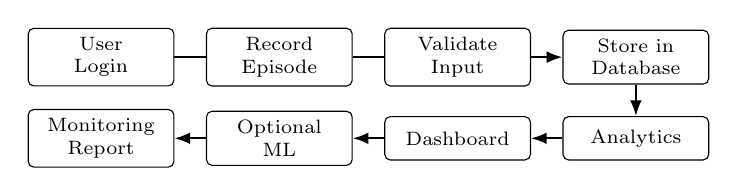
\begin{tikzpicture}[node distance=4mm]
\node[smallbox] (login) {User\\Login};
\node[smallbox,right=of login] (record) {Record\\Episode};
\node[smallbox,right=of record] (valid) {Validate\\Input};
\node[smallbox,right=of valid] (store) {Store in\\Database};
\node[smallbox,below=of store] (ana) {Analytics};
\node[smallbox,left=of ana] (dash) {Dashboard};
\node[smallbox,left=of dash] (ml) {Optional\\ML};
\node[smallbox,left=of ml] (report) {Monitoring\\Report};
\draw[arrow] (login)--(record)--(valid)--(store);
\draw[arrow] (store)--(ana);
\draw[arrow] (ana)--(dash);
\draw[arrow] (dash)--(ml);
\draw[arrow] (ml)--(report);
\end{tikzpicture}
\captionof{figure}{End-to-end operational workflow.}
\end{center}



\section{Episode Data Collection}

Each episode records date/time, severity, duration, affected body area, activity, self-reported stress, possible trigger, temperature and humidity where available, and additional notes.

\begin{center}
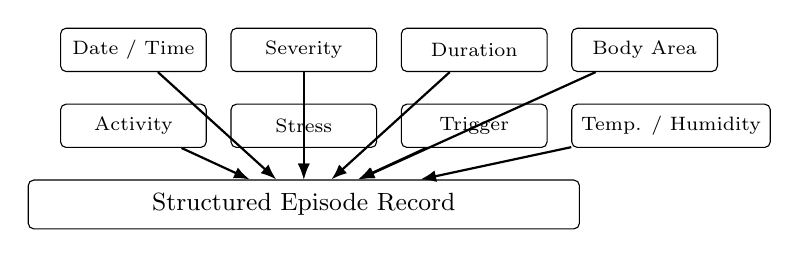
\begin{tikzpicture}[node distance=4mm and 3mm]
\node[smallbox] (time) {Date / Time};
\node[smallbox,right=of time] (sev) {Severity};
\node[smallbox,right=of sev] (dur) {Duration};
\node[smallbox,right=of dur] (area) {Body Area};
\node[smallbox,below=of time] (act) {Activity};
\node[smallbox,right=of act] (stress) {Stress};
\node[smallbox,right=of stress] (trig) {Trigger};
\node[smallbox,right=of trig] (env) {Temp. / Humidity};
\node[box,below=of stress,minimum width=7.0cm] (record) {Structured Episode Record};
\draw[arrow] (time)--(record);
\draw[arrow] (sev)--(record);
\draw[arrow] (dur)--(record);
\draw[arrow] (area)--(record);
\draw[arrow] (act)--(record);
\draw[arrow] (stress)--(record);
\draw[arrow] (trig)--(record);
\draw[arrow] (env)--(record);
\end{tikzpicture}
\captionof{figure}{Structured data captured for each episode.}
\end{center}

\section{Data Processing and Analytics}

Records are cleaned and processed to derive daily/weekly frequency, average severity, average duration, frequently affected areas, common possible triggers, severity trends, and associations between recorded stress and severity.

\begin{center}
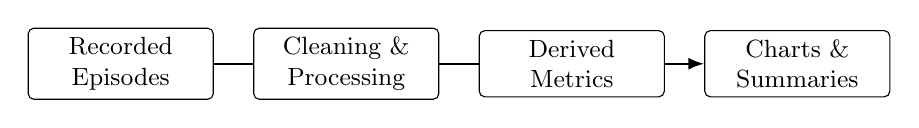
\begin{tikzpicture}[node distance=5mm]
\node[box] (raw) {Recorded\\Episodes};
\node[box,right=of raw] (clean) {Cleaning \&\\Processing};
\node[box,right=of clean] (metric) {Derived\\Metrics};
\node[box,right=of metric] (view) {Charts \&\\Summaries};
\draw[arrow] (raw)--(clean)--(metric)--(view);
\end{tikzpicture}
\captionof{figure}{Analytics pipeline and derived metrics.}
\end{center}

\section{Machine Learning Component}

The AIML component investigates supervised severity classification. Candidate features include stress, temperature, humidity, activity, time of day, previous severity, duration, caffeine intake, and affected body area. Candidate algorithms are Logistic Regression, Decision Trees, and Random Forest; the target is \textbf{Low / Moderate / High}.

\begin{center}
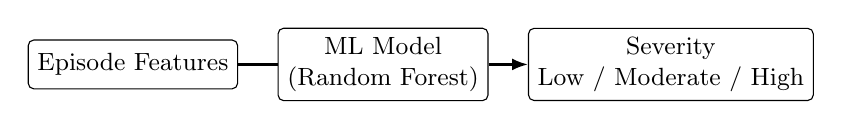
\begin{tikzpicture}[node distance=5mm]
\node[box] (features) {Episode Features};
\node[box,right=of features] (model) {ML Model\\(Random Forest)};
\node[box,right=of model] (out) {Severity\\Low / Moderate / High};
\draw[arrow] (features)--(model)--(out);
\end{tikzpicture}
\captionof{figure}{Proposed machine learning pipeline.}
\end{center}


\section{Testing and Validation}

Testing is performed throughout development.

\begin{itemize}
\item \textbf{Unit Testing:} login, episode creation, validation and individual functions.
\item \textbf{Integration Testing:} frontend, backend, database and analytics communication.
\item \textbf{System Testing:} complete workflow from login to report generation.
\item \textbf{User Acceptance Testing:} usability and clarity evaluation.
\item \textbf{ML Evaluation:} accuracy, precision, recall, F1-score and confusion matrix, if ML is implemented.
\end{itemize}

\begin{center}

\begin{tikzpicture}[node distance=5mm]
\node[smallbox] (unit) {Unit};
\node[smallbox,right=of unit] (int) {Integration};
\node[smallbox,right=of int] (sys) {System};
\node[smallbox,right=of sys] (uat) {User\\Acceptance};
\node[smallbox,right=of uat] (mlt) {ML\\Evaluation};
\draw[arrow] (unit)--(int)--(sys)--(uat)--(mlt);
\end{tikzpicture}
\captionof{figure}{Multi-level testing and validation strategy.}
\end{center}

\section{Technology Stack}

\begin{center}
\begin{tabular}{>{\bfseries}p{0.27\textwidth}p{0.55\textwidth}}
\toprule
Component & Technology\\
\midrule
Frontend & HTML, CSS, JavaScript\\
Backend & Python, Flask, REST API\\
Database & MySQL\\
Data Processing & Pandas, NumPy\\
Machine Learning & Scikit-learn\\
Visualization & Chart.js / Matplotlib\\
Testing & Python testing framework\\
Version Control & Git and GitHub\\
Development & VS Code / PyCharm\\
\bottomrule
\end{tabular}
\end{center}

\begin{center}
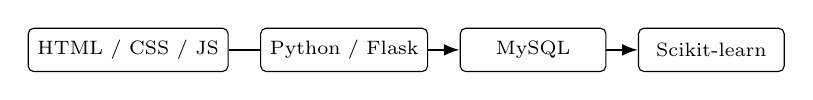
\begin{tikzpicture}[node distance=4mm]
\node[smallbox] (fe) {HTML / CSS / JS};
\node[smallbox,right=of fe] (be) {Python / Flask};
\node[smallbox,right=of be] (db) {MySQL};
\node[smallbox,right=of db] (ml) {Scikit-learn};
\draw[arrow] (fe)--(be)--(db);
\draw[arrow] (db)--(ml);
\end{tikzpicture}
\captionof{figure}{Technology stack across the application.}
\end{center}

\section{Development Timeline}

\begin{center}
\small
\begin{tabular}{p{0.14\textwidth}p{0.47\textwidth}p{0.28\textwidth}}
\toprule
\textbf{Weeks} & \textbf{Task} & \textbf{Deliverable}\\
\midrule
1--2 & Requirements and problem study & SRS\\
3--4 & Architecture and database design & Architecture + ER/UML\\
5--6 & Frontend and authentication & Working interface\\
7--8 & Episode recording + database & Monitoring module\\
9--10 & Dashboard + analytics & Charts and trends\\
11 & Treatment tracking + reports & Report module\\
12 & ML investigation & Prediction prototype\\
13 & Integration + system testing & Test results\\
14 & User acceptance + refinement & Validated prototype\\
15 & Documentation + presentation & Final report\\
\bottomrule
\end{tabular}
\end{center}


\section{Resources and Budget}

The project is developed by two students. Aditya Rajput focuses on backend development, database integration, ML, and system integration. Prabhkirat Kaur focuses on frontend development, UI/UX, documentation, testing, and analytics integration. Both participate in requirements, design, testing, and final documentation.

The project primarily uses freely available/open-source software: Python, Flask, MySQL, Pandas, NumPy, Scikit-learn, HTML/CSS/JavaScript, Git/GitHub, and VS Code/PyCharm. No external funding is required for the initial implementation.

\section{Risks and Mitigation}

\begin{itemize}
\item \textbf{Limited data:} use suitable public/synthetic data for the ML prototype and consider anonymized data in future.
\item \textbf{Data privacy:} collect only necessary information and protect it through authentication and database security.
\item \textbf{Medical interpretation:} clearly position the system as monitoring/analysis, not diagnosis or treatment.
\item \textbf{ML reliability:} present predictions only as supplementary insights.
\item \textbf{Development delays:} prioritize core monitoring before advanced ML.
\item \textbf{User adoption:} keep episode recording quick and simple.
\end{itemize}

\begin{center}
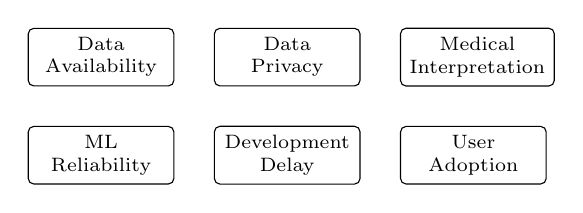
\begin{tikzpicture}[node distance=5mm and 5mm]
\node[smallbox] (data) {Data\\Availability};
\node[smallbox,right=of data] (privacy) {Data\\Privacy};
\node[smallbox,right=of privacy] (medical) {Medical\\Interpretation};
\node[smallbox,below=of data] (mlrisk) {ML\\Reliability};
\node[smallbox,right=of mlrisk] (delay) {Development\\Delay};
\node[smallbox,right=of delay] (adopt) {User\\Adoption};
\end{tikzpicture}
\captionof{figure}{Key project risks.}
\end{center}

\section{Expected Outcomes}

At completion, HyperTrack is expected to provide:

\begin{itemize}
\item structured episode records and historical views;
\item frequency, severity and trigger trends;
\item treatment/session history;
\item organized monitoring reports; and
\item optional ML-based personalized severity insights.
\end{itemize}

\begin{center}
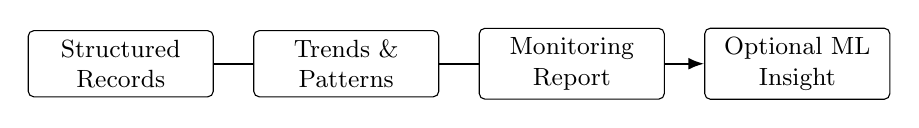
\begin{tikzpicture}[node distance=5mm]
\node[box] (records) {Structured\\Records};
\node[box,right=of records] (trends) {Trends \&\\Patterns};
\node[box,right=of trends] (report) {Monitoring\\Report};
\node[box,right=of report] (insight) {Optional ML\\Insight};
\draw[arrow] (records)--(trends)--(report)--(insight);
\end{tikzpicture}
\captionof{figure}{Expected project outcomes.}
\end{center}

\section{Summary}

HyperTrack is a software-based monitoring and management system for organizing and analyzing hyperhidrosis-related sweating episodes. It combines structured data collection, database management, visualization, reporting, and an optional AIML component for severity prediction. The project emphasizes requirements engineering, modular architecture, testing, usability, privacy, and scalability.

\textbf{Clinical Scope Note:} HyperTrack is a monitoring and decision-support system. Its analytics and ML outputs are supplementary insights from user-recorded data and are not medical diagnosis, treatment recommendations, or medical advice.

\vspace{8pt}
\begin{center}
Aditya Rajput --- Roll No: 1024240145 --- arajput\_be24@thapar.edu\\
Prabhkirat Kaur --- Roll No: 1024240024 --- pkaur2\_be24@thapar.edu
\end{center}

\end{document}
